
\section{\LSEQ : une fonction d'allocation polylogarithmique}
\label{repl:sec:proposal}

\LSEQ (\emph{polyLogarithmic SEQuence}) est une fonction d'allocation
d'identifiants de taille variable pour les structures de données sans résolution
de conflits dédiées aux séquences. \LSEQ est composée de trois éléments dont les
comportements, pris individuellement, n'arrivent pas à pourvoir des identifiants
de taille satisfaisante. En revanche, utilisés simultanément, les défaillances
des uns sont comblées par les forces des autres. En résulte une allocation
d'identifiants dont la borne supérieure sur la taille est polylogarithmique
comparé au nombre d'insertions effectuées dans le document. 
L'idée générale de \LSEQ consiste à accepter la perte de niveaux des chemins
composants ses identifiants pour peu que les allocations suivantes réparent les
dommages.

Le premier composant est un structure d'arbre dont l'arité augmente avec sa
profondeur (cf. §\ref{repl:subsec:exponentialtree}). L'intuition étant que si la
profondeur de l'arbre augmente, c'est que le document à grandit suffisamment
pour nécessiter un plus large champs d'identifiants. Mais au lieu d'ouvrir un
espace aussi large qu'auparavant, l'espace est élargi afin que le document
puisse se satisfaire de ce champs d'identifiants plus longuement.

Le second composant comprend deux sous-fonctions d'allocation conçues pour gérer
des comportements d'édition opposés (cf. §\ref{repl:subsec:suballocation}). Ainsi,
l'une est appropriée lorsque l'édition est principalement faite de gauche à
droite tandis que l'autre cible l'édition de droite à gauche. Elles seront
utilisées ensemble afin de pouvoir gérer la plupart des cas d'édition.

Le troisième composant est une fonction assignant à chaque profondeur de l'arbre
une sous-fonction d'allocation parmi celles disponibles
(cf. §\ref{repl:subsec:allocationchoice}). Cette fonction de choix doit fournir des
réponses similaires quelle que soit la réplique.

\subsection{Arbre exponentiel}
\label{repl:subsec:exponentialtree}

Un arbre exponentiel est une structure d'arbre dont chacun des nœuds possède une
arité maximale $k$ fois supérieure à celle de son parent. Ainsi, la progression
du nombre de fils dans une branche est exponentielle. Un chemin dans un tel
arbre nécessite nécessite un bit additionnel par concaténation.

\begin{figure}
  \begin{center}
    \input{input/replication/figexponentialtree.tex}
    \caption{\label{repl:fig:exponentialtree}Arbre exponentiel.}
  \end{center}
\end{figure}

La figure~\ref{repl:fig:exponentialtree} montre un arbre exponentiel. L'arbre
commence avec une arité maximale de 2. Puis chacun de ces fils a une arité
maximale de 4. Puis chacun de ces fils a une arité maximale de 8. Un chemin de
profondeur 3 tel que [1.3.7] nécessite alors 1+2+3 = 6 bits pour sa
représentation en mémoire.

Plus généralement, un chemin de profondeur $e$ requière
$\textstyle\sum\nolimits_{i=1}^{e}i = {e^2 + e \over{2}}$ bits. Cette progression
quadratique en fonction de la profondeur rend essentielle la prise en charge des
comportements d'édition conduisant au pire cas
(cf. figure~\ref{repl:fig:allocpathexampleB}). En particulier, un comportement
aussi simple que l'édition de droite à gauche doit impérativement être géré
(cf. figure~\ref{repl:img:motivationsB}).

\subsection{Sous-fonctions d'allocation}
\label{repl:subsec:suballocation}

L'allocation d'identifiants optimale suppose de connaître le nombre et la
position des éditions successives. Avec cette connaissance, les identifiants
auraient une croissance logarithmique comparée à la taille
document. Malheureusement, aucune de ces deux informations n'est disponible dans
l'édition collaborative en temps réel.

Dans ces conditions, nous supposerons que le comportement d'édition est une
suite d'éditions adjacentes les unes des autres -- comme l'édition en tête ou
l'édition en fin -- ou à des positions aléatoires, ou enfin, une composition de
ceux-ci.

\begin{figure}
  \begin{center}
    \subfloat[Sous-fonction d'allocation conçue pour l'édition de gauche à droite]
    [\label{repl:fig:suballocationA}\TODO{Sous-fonction d'allocation conçue 
    pour l'édition de gauche à droite}]
    {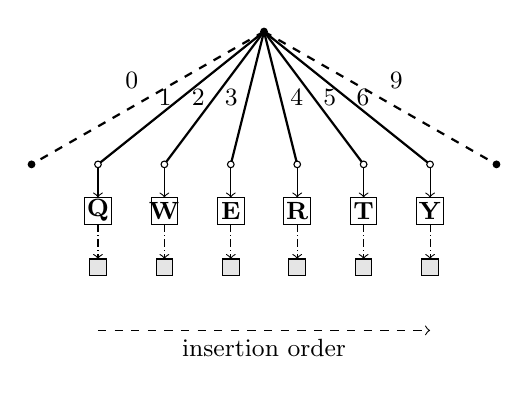
\begin{tikzpicture}[scale=1.2]

  %% node to node
  \small
  \draw[dashed, thick] (0pt,0pt) -- node[anchor=south east]{0} (-70pt,-40pt);
  \draw[thick] (0pt,0pt) -- node[anchor=east]{\DARKBLUE{1}} (-50pt,-40pt);
  \draw[thick] (0pt,0pt) -- node[anchor=east]{\DARKBLUE{2}} (-30pt,-40pt);
  \draw[thick] (0pt,0pt) -- node[anchor=east]{\DARKBLUE{3}} (-10pt,-40pt);
  \draw[thick] (0pt,0pt) -- node[anchor=west]{\DARKBLUE{4}} ( 10pt,-40pt);
  \draw[thick] (0pt,0pt) -- node[anchor=west]{\DARKBLUE{5}} ( 30pt,-40pt);
  \draw[thick] (0pt,0pt) -- node[anchor=west]{\DARKBLUE{6}} ( 50pt,-40pt);
  \draw[dashed, thick] (0pt,0pt) -- node[anchor=south west]{9} ( 70pt,-40pt);

  %% node to element
  \draw[->] (-50pt,-40pt) -- (-50pt,-50pt);
  \draw[->] (-30pt,-40pt) -- (-30pt,-50pt);
  \draw[->] (-10pt,-40pt) -- (-10pt,-50pt);
  \draw[->] ( 10pt,-40pt) -- ( 10pt,-50pt);
  \draw[->] ( 30pt,-40pt) -- ( 30pt,-50pt);
  \draw[->] ( 50pt,-40pt) -- ( 50pt,-50pt);

  %% element to desambiguator
  \draw[->,densely dashdotted] ( -50pt,-58pt) -- ( -50pt,-68.5pt);
  \draw[->,densely dashdotted] ( -30pt,-58pt) -- ( -30pt,-68.5pt);
  \draw[->,densely dashdotted] ( -10pt,-58pt) -- ( -10pt,-68.5pt);
  \draw[->,densely dashdotted] (  10pt,-58pt) -- (  10pt,-68.5pt);
  \draw[->,densely dashdotted] (  30pt,-58pt) -- (  30pt,-68.5pt);
  \draw[->,densely dashdotted] (  50pt,-58pt) -- (  50pt,-68.5pt);

  \draw[fill=black] (  0pt,  0pt) circle (1pt);
  \draw[fill=black] (-70pt,-40pt) circle (1pt);
  \draw[fill=white] (-50pt,-40pt) circle (1pt);
  \draw[fill=white] (-30pt,-40pt) circle (1pt);
  \draw[fill=white] (-10pt,-40pt) circle (1pt);
  \draw[fill=white] ( 10pt,-40pt) circle (1pt);
  \draw[fill=white] ( 30pt,-40pt) circle (1pt);
  \draw[fill=white] ( 50pt,-40pt) circle (1pt);
  \draw[fill=black] ( 70pt,-40pt) circle (1pt);

  %% elements
  \draw[fill=white](-50pt,-54pt)
  node{\textbf{Q}}+(-4pt,-4pt)rectangle+(4pt,4pt) ;
  \draw[fill=white](50pt,-54pt)
  node{\textbf{Y}} +(-4pt,-4pt) rectangle +(4pt,4pt) ;
  \draw[fill=white]( 10pt,-54pt)
  node{\textbf{R}} +(-4pt,-4pt) rectangle +(4pt,4pt) ;
  \draw[fill=white] ( -30pt,-54pt)
  node{\textbf{W}} +(-4pt,-4pt) rectangle +(4pt,4pt) ;
  \draw[fill=white] ( -10pt,-54pt)
  node{\textbf{E}} +(-4pt,-4pt) rectangle +(4pt,4pt) ;
  \draw[fill=white]( 30pt,-54pt)
  node{\textbf{T}} +(-4pt,-4pt) rectangle +(4pt,4pt) ;

  %% desambiguator
  \draw[fill=gray!20] (-50pt,-71pt) +(-2.5pt,-2.5pt) rectangle +(2.5pt,2.5pt);
  \draw[fill=gray!20] (-30pt,-71pt) +(-2.5pt,-2.5pt) rectangle +(2.5pt,2.5pt);
  \draw[fill=gray!20] (-10pt,-71pt) +(-2.5pt,-2.5pt) rectangle +(2.5pt,2.5pt);
  \draw[fill=gray!20] ( 10pt,-71pt) +(-2.5pt,-2.5pt) rectangle +(2.5pt,2.5pt);
  \draw[fill=gray!20] ( 30pt,-71pt) +(-2.5pt,-2.5pt) rectangle +(2.5pt,2.5pt);
  \draw[fill=gray!20] ( 50pt,-71pt) +(-2.5pt,-2.5pt) rectangle +(2.5pt,2.5pt);

  %% insertion order
  \draw[->,dashed] (-50pt, -90pt) -- node[anchor=north]{insertion order}
  (50pt, -90pt);

\end{tikzpicture}
}
    \hspace{20pt}
    \subfloat[Sous-fonction d'allocation conçue pour l'édition de droite à gauche]
    [\label{repl:fig:suballocationB}\TODO{Sous-fonction d'allocation conçue
    pour l'édition de droite à gauche}]
    {\input{input/replication/figsuballocationB.tex}}
    \caption{Deux sous-fonctions d'allocation.}
  \end{center}
\end{figure}

Afin de gérer ces types d'édition, employer une fonction d'allocation conçue
pour l'édition en fin ne suffit pas. \TODO{Moar. Talk about boundary.}

\subsection{Choix de sous-fonction d'allocation}
\label{repl:subsec:allocationchoice}

L'emploi de plusieurs sous-fonctions d'allocation oblige à choisir parmi
celle-ci. Cela pose deux problèmes, à savoir,
\begin{inparaenum}[(i)]
\item quel événement déclanche une prise de décision, et lorsque cela survient, 
\item quelle sous-fonction employer.
\end{inparaenum}


\subsection{Résumé}

\begin{figure}
  \begin{center}
    \subfloat[Édition de gauche à droite dans \LSEQ]
    [Édition de gauche à droite dans \LSEQ]
    {\input{input/replication/figlseqtreeexampleA.tex}}
    \subfloat[Édition de droite à gauche dans \LSEQ]
    [Édition de droite à gauche dans \LSEQ]
    {\input{input/replication/figlseqtreeexampleB.tex}}
    \caption{\TODO{Meow}}
  \end{center}
\end{figure}


%%% Local Variables:
%%% mode: latex
%%% TeX-master: "../../paper"
%%% End:
